% !TeX program  = xelatex
% !TeX encoding = UTF-8
% !TeX root     = article1.tex
\documentclass{../mirea}

% !TeX program  = xelatex
% !TeX encoding = UTF-8
% !TeX root     = article1.tex

\usepackage{hyperref}
\hypersetup{pdftitle={ВКР на тему "<Разработка системы для поиска и возврата утерянных вещей">}, pdfauthor={В. С. Верхотуров}}

\usepackage{comment}

\usepackage{graphicx}

\usepackage{listings}
\usepackage{xcolor}
\lstset{basicstyle=\footnotesize, breaklines=true, numbers=left, captionpos=t, showstringspaces=false, commentstyle=\color{teal}, stringstyle=\color{red}, keywordstyle=\color{violet}}  % Настройки, применяемые ко всем листингам

% Создание введения или заключения
\newcommand{\supersection}[1]{
	\section*{#1}
	\phantomsection
	\addcontentsline{toc}{section}{#1}
}

\usepackage{caption}
\captionsetup[lstlisting]{justification=raggedright, singlelinecheck=false}

\usepackage{pdfpages}

\usepackage{microtype}

\usepackage{multirow}

\usepackage{array}
\usepackage{setspace}
\newcolumntype{x}[1]{>{\setstretch{0.8}\small\centering\arraybackslash\hspace{0pt}}m{#1}}
\newcolumntype{y}[1]{>{\centering\arraybackslash\hspace{0pt}}m{#1}}
\usepackage{longtable}

\usepackage{float}

%\usepackage{color,xesearch}
%\SearchList{make-red}{\textcolor{red}{#1}}{эффективность,эффективности,эффективностью,эффективностей,эффективностям,эффективностями,эффективностях,эффективный,эффективная,эффективное,инновационный,иновационная,иновационные,инновация,иновационных,надежность,оптимизация,качество}


\begin{document}
	
	% 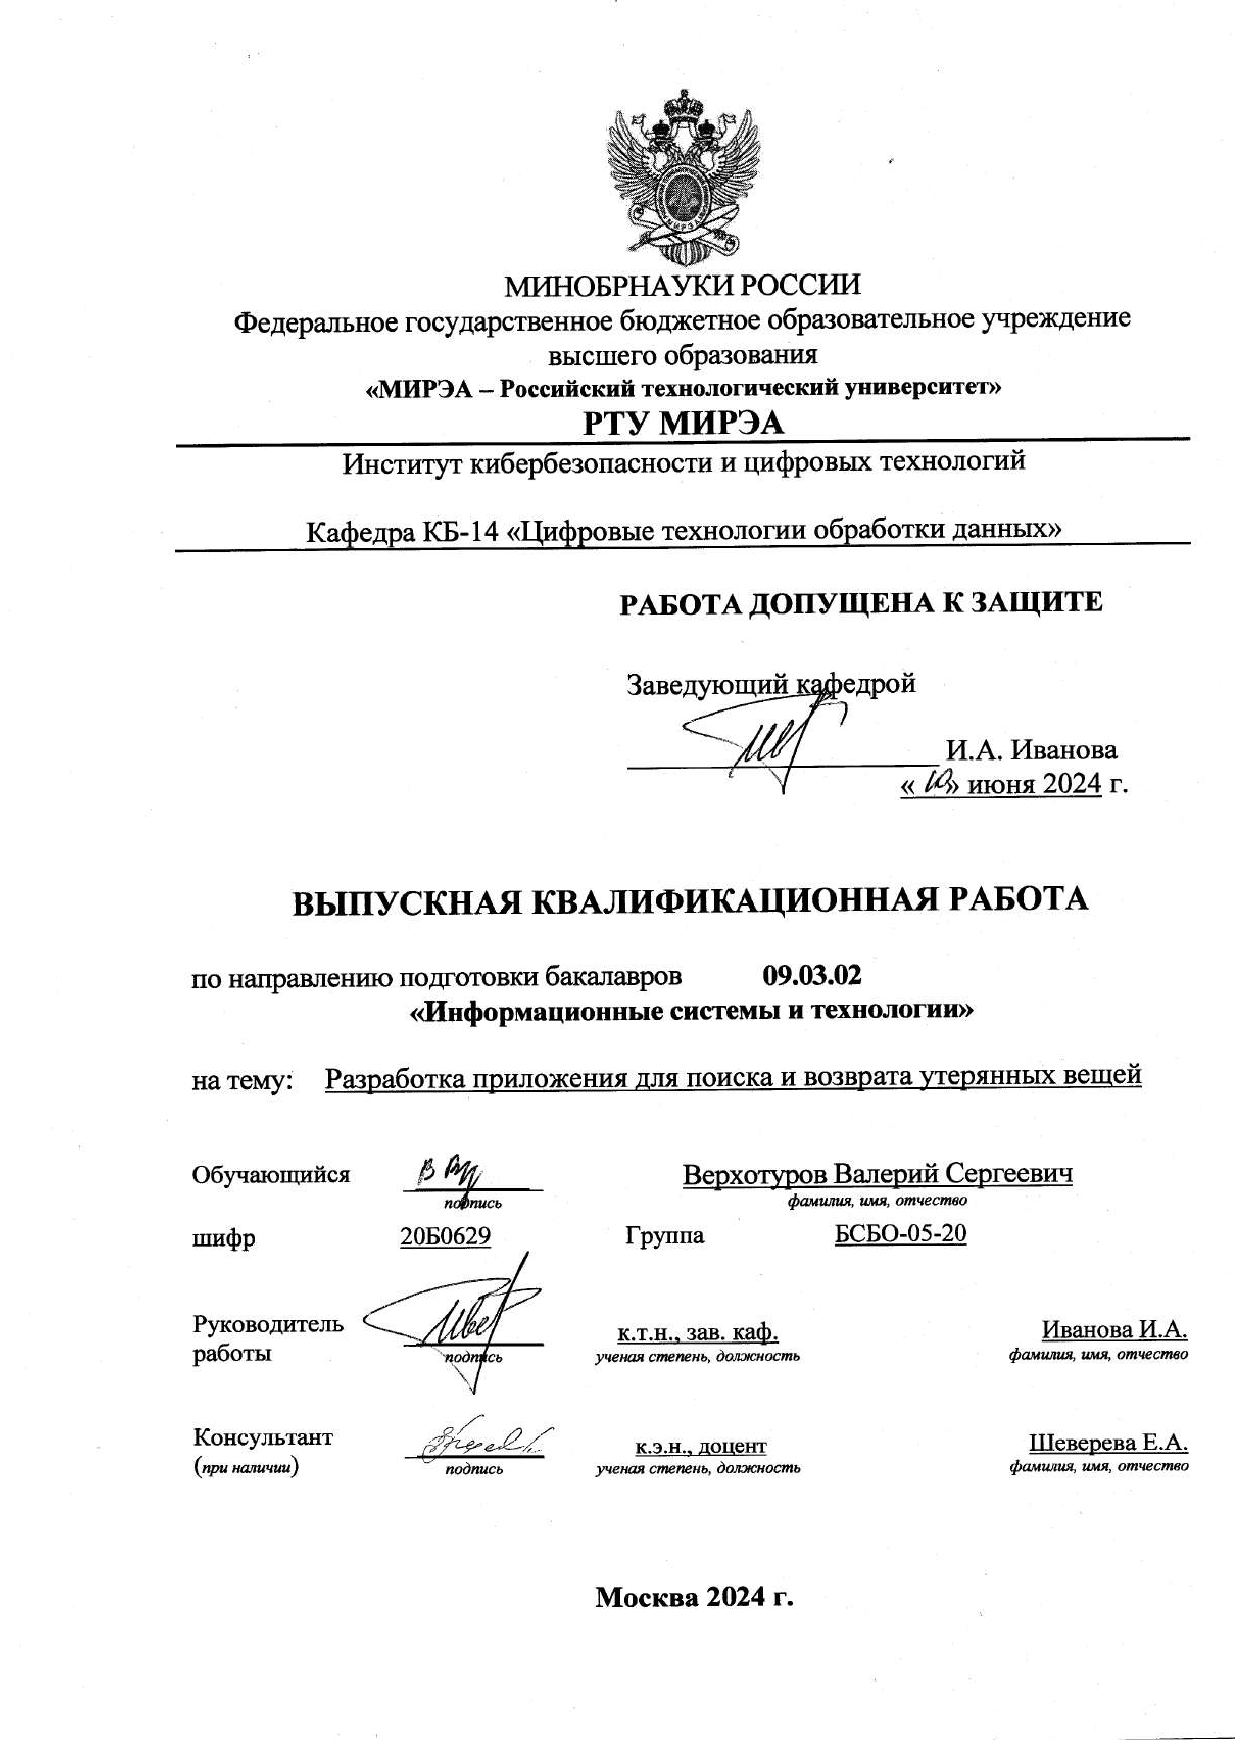
\includepdf[pages=-]{titlepage.pdf}
	
	\addtocounter{page}{2}
	
	% Содержание
	\tableofcontents
	
	\supersection{Введение}
	\label{sec:introduction}
	
	Поиск утерянных вещей является актуальной проблемой, которая возникает при различных обстоятельствах. Эта проблема может возникнуть в результате потери ключей, документов, мобильных телефонов, кошельков или других ценных или важных вещей~\cite{bib:m24_losts_article,bib:usinsk_losts_article}. В связи с этим существует необходимость разработки системы, которая поможет людям вернуть утерянные вещи.
	
	Целью данной работы является проведение анализа существующих систем поиска утерянных вещей и выделение их преимуществ и недостатков.
	
	\section{Статистика потерянных и найденных вещей}
	
	Для подтверждения актуальности и важности разрабатываемой системы, необходимо провести исследование рынка и определить основные проблемы и потребности пользователей. Одним из способов сбора информации является проведение опроса среди пользователей.
	
	Одним из основных факторов, определяющих актуальность разрабатываемой системы является статистика потерянных и найденных вещей. Необходимо определить количество потерянных вещей в месяц, год и за весь период работы системы. Это поможет оценить нагрузку на систему и определить ее производительность.
	
	Статистика, взятая с сайта столнаходок.рф~\cite{bib:stol_nahodok}, утверждает, что только 20~\% пользователей их сайта смогли установить и вернуть вещи. Также на рисунках \ref{fig:chart2023} и \ref{fig:chart2022} представлена гистограмма количества созданных объявлений за 2022 и 2023 года.
	
	\begin{figure}[htb]
		\centering
		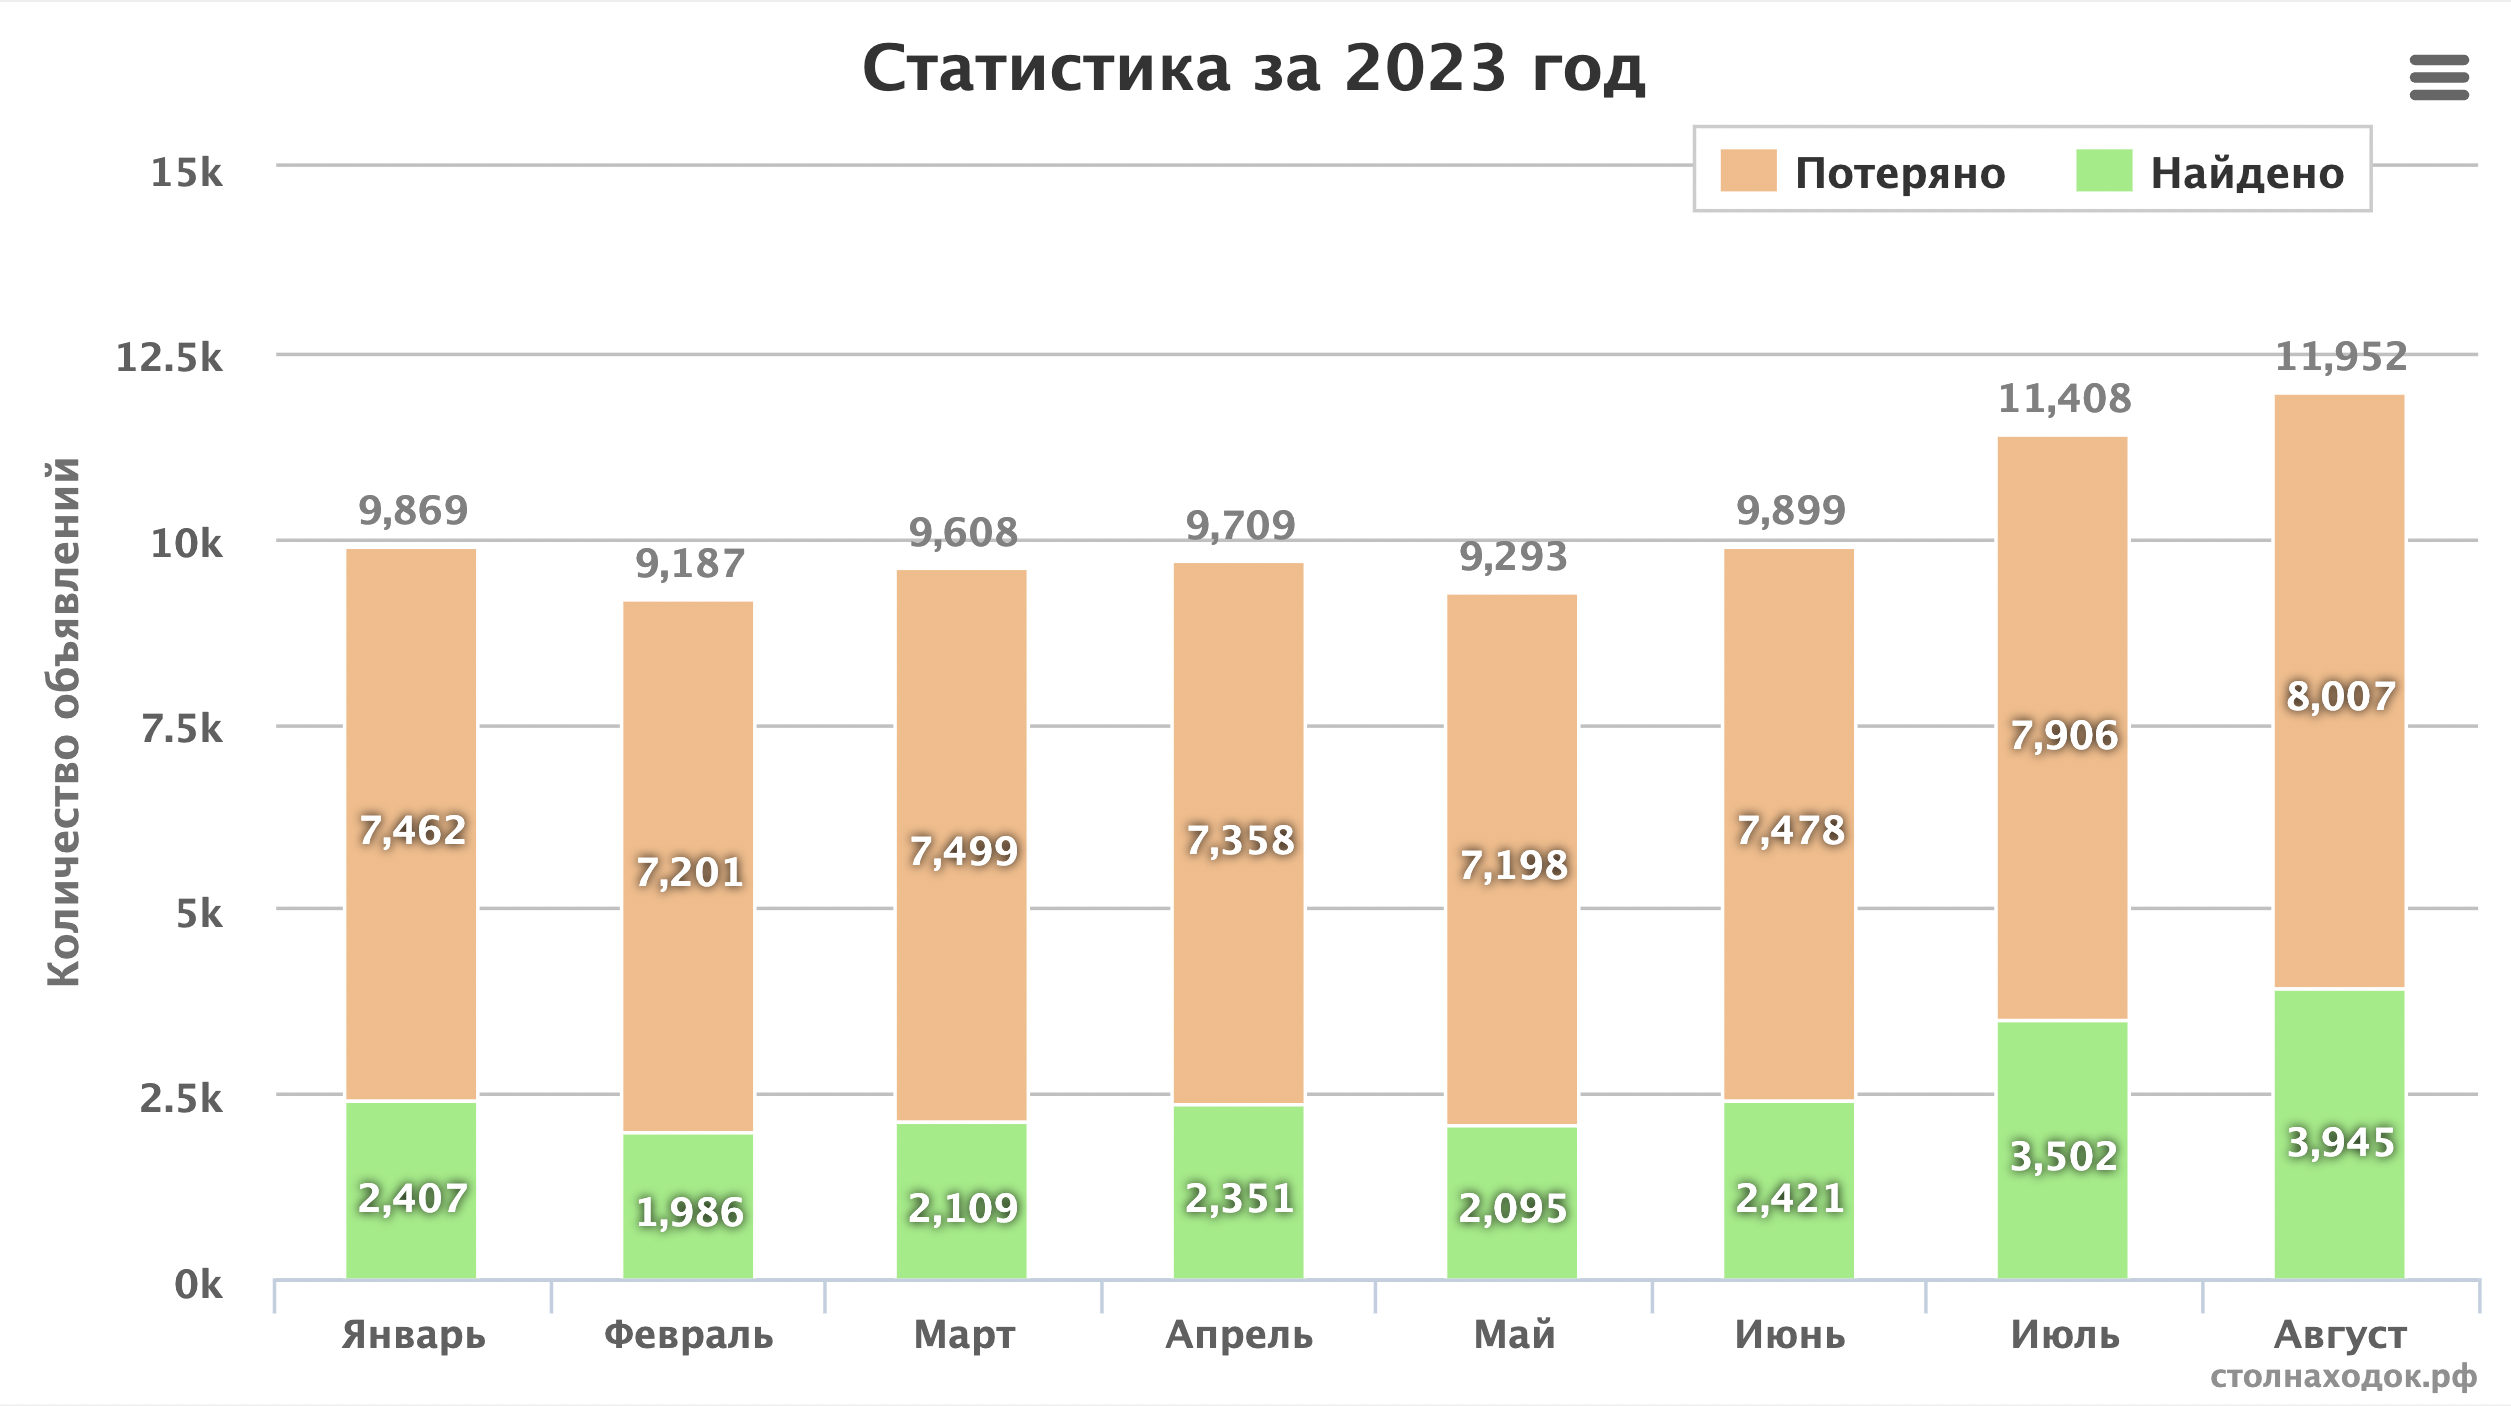
\includegraphics[width=.6\textwidth]{../images/chart2023}
		\parskip=6pt
		\caption{Востребованность системы столнаходок.рф в 2023 году}
		\label{fig:chart2023}
	\end{figure}
	
	\begin{figure}[htb]
		\centering
		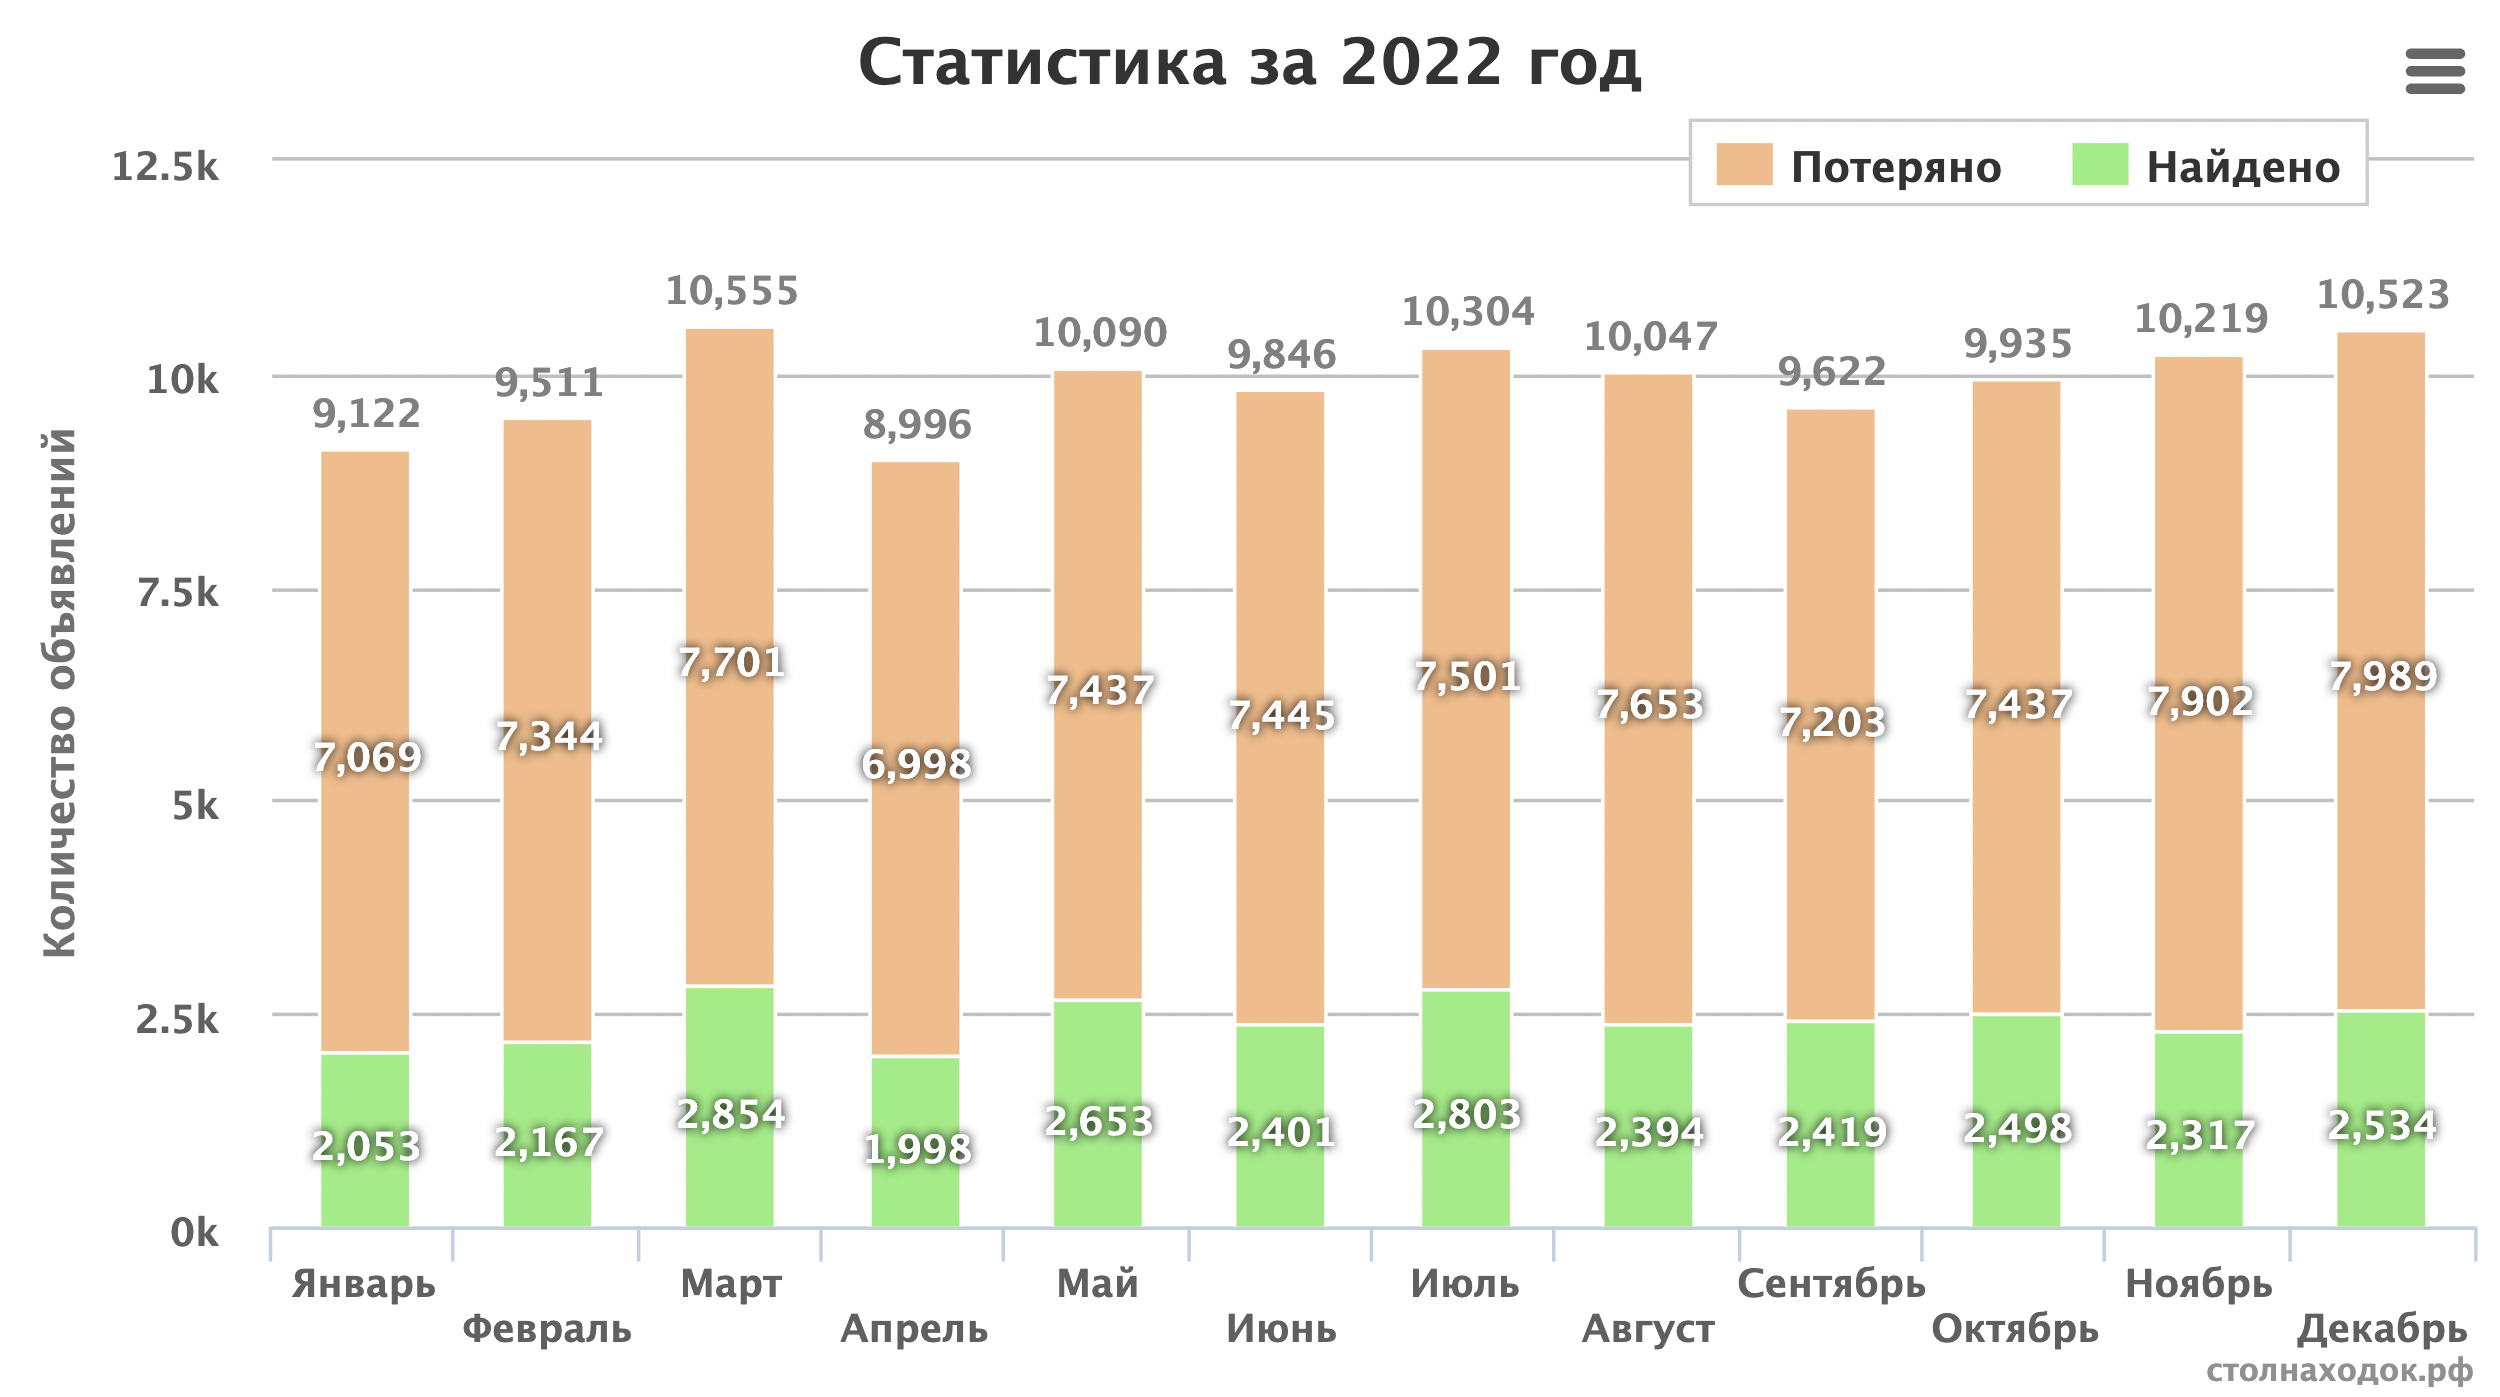
\includegraphics[width=.6\textwidth]{../images/chart2022}
		\parskip=6pt
		\caption{Востребованность системы столнаходок.рф в 2022 году}
		\label{fig:chart2022}
	\end{figure}
	
	\section{Типы существующих решений для поиска и возврата утерянных вещей}
	
	Существует несколько типов существующих решений для поиска и возврата утерянных вещей. Ниже приведены некоторые из них:
	\begin{enumerate}
		\item Веб-сайты и мобильные приложения: <<Бюро находок>>~\cite{bib:stol_nahodok,bib:pona}. Эти сервисы предоставляют платформу, где люди могут регистрировать утерянные вещи и искать их владельцев. Пользователям предлагается создать объявления о найденных или потерянных вещах и связаться друг с другом, чтобы вернуть вещи. Некоторые сервисы предлагают добавить фотографии или описание вещей, чтобы облегчить поиск. 
		
		\item Технология RFID (Radio Frequency Identification) позволяет прикреплять RFID-метки к ценным объектам и определить владельца с помощью специальных считывателей~\cite{bib:investopedia_rfid,bib:airtag}. Это возможно благодаря использованию радиоволн, которые позволяют быстро определять местоположение потерянных вещей с помощью дополнительного программного обеспечения. Одним из наиболее распространенных применений технологии RFID является микрочипирование домашних животных или чипов для домашних животных. Эти микрочипы имплантируются ветеринарами и содержат информацию, касающуюся домашних животных, включая их имя, медицинские записи и контактную информацию их владельцев. Если домашнее животное пропадает и его отправляют в спасательную службу или в приют, работник приюта сканирует животное на наличие микрочипа. Если у домашнего животного есть микрочип, работнику приюта достаточно одного телефонного звонка или поиска в Интернете, чтобы связаться с владельцами домашнего животного. Считается, что чипы для домашних животных более надежны, чем ошейники, которые можно упасть или снять.
		
		\item GPS-трекеры --- это устройства с встроенным GPS-модулем. Они могут быть прикреплены практически к любому объекту, после чего его местоположение определяется через смартфон или компьютер по сети Интернет. При использовании приложения на смартфоне пользователь может получать уведомления о передвижении объекта и быстро определять его текущее местоположение.
		
		\item Автоматизированные системы поиска утерянных предметов: Некоторые организации, например, аэропорты и железнодорожные станции, используют системы обнаружения утерянных предметов. В этих системах используются технологии, такие как видеонаблюдение, детекторы движения и распознавание образов для отслеживания и возвращения потерянных предметов их владельцам.
	\end{enumerate}
	
	Каждый из этих типов решений имеет свои преимущества и недостатки. Некоторые из них могут быть более подходящими для конкретных ситуаций, например, GPS-трекеры могут быть полезными при поиске утерянных вещей на открытой местности, в то время как RFID-метки могут быть более подходящими для использования внутри помещений. Веб-сайты и приложения <<Бюро находок>> предоставляют более универсальное решение, которое может быть использовано в различных ситуациях.
	
	\section{Анализ существующих систем для поиска и возврата утерянных вещей}
	
	В настоящем разделе будет проведен обзор существующих сервисов и приложений, которые предлагают функциональность поиска и возврата утерянных вещей. Данный обзор позволит выявить основные преимущества и недостатки этих сервисов, а также определить потенциальные возможности для улучшения их функциональности.
	
	<<столнаходок.рф>>~\cite{bib:stol_nahodok} --- это один из наиболее популярных веб-сервисов, предоставляющих возможность объявлять о потерянных и найденных предметах. Сервис имеет простой и интуитивно понятный интерфейс, позволяющий пользователям быстро разместить информацию о потерянных вещах и связаться с владельцами найденных предметов, примеры пользовательского интерфейса представлены на рис.~\ref{fig:stolNahodok1}, \ref{fig:stolNahodok2}. Однако, отсутствие системы уведомлений и неудобное сопоставление объявлений ограничивают его функциональность.
	
	\begin{figure}[htb]
		\centering
		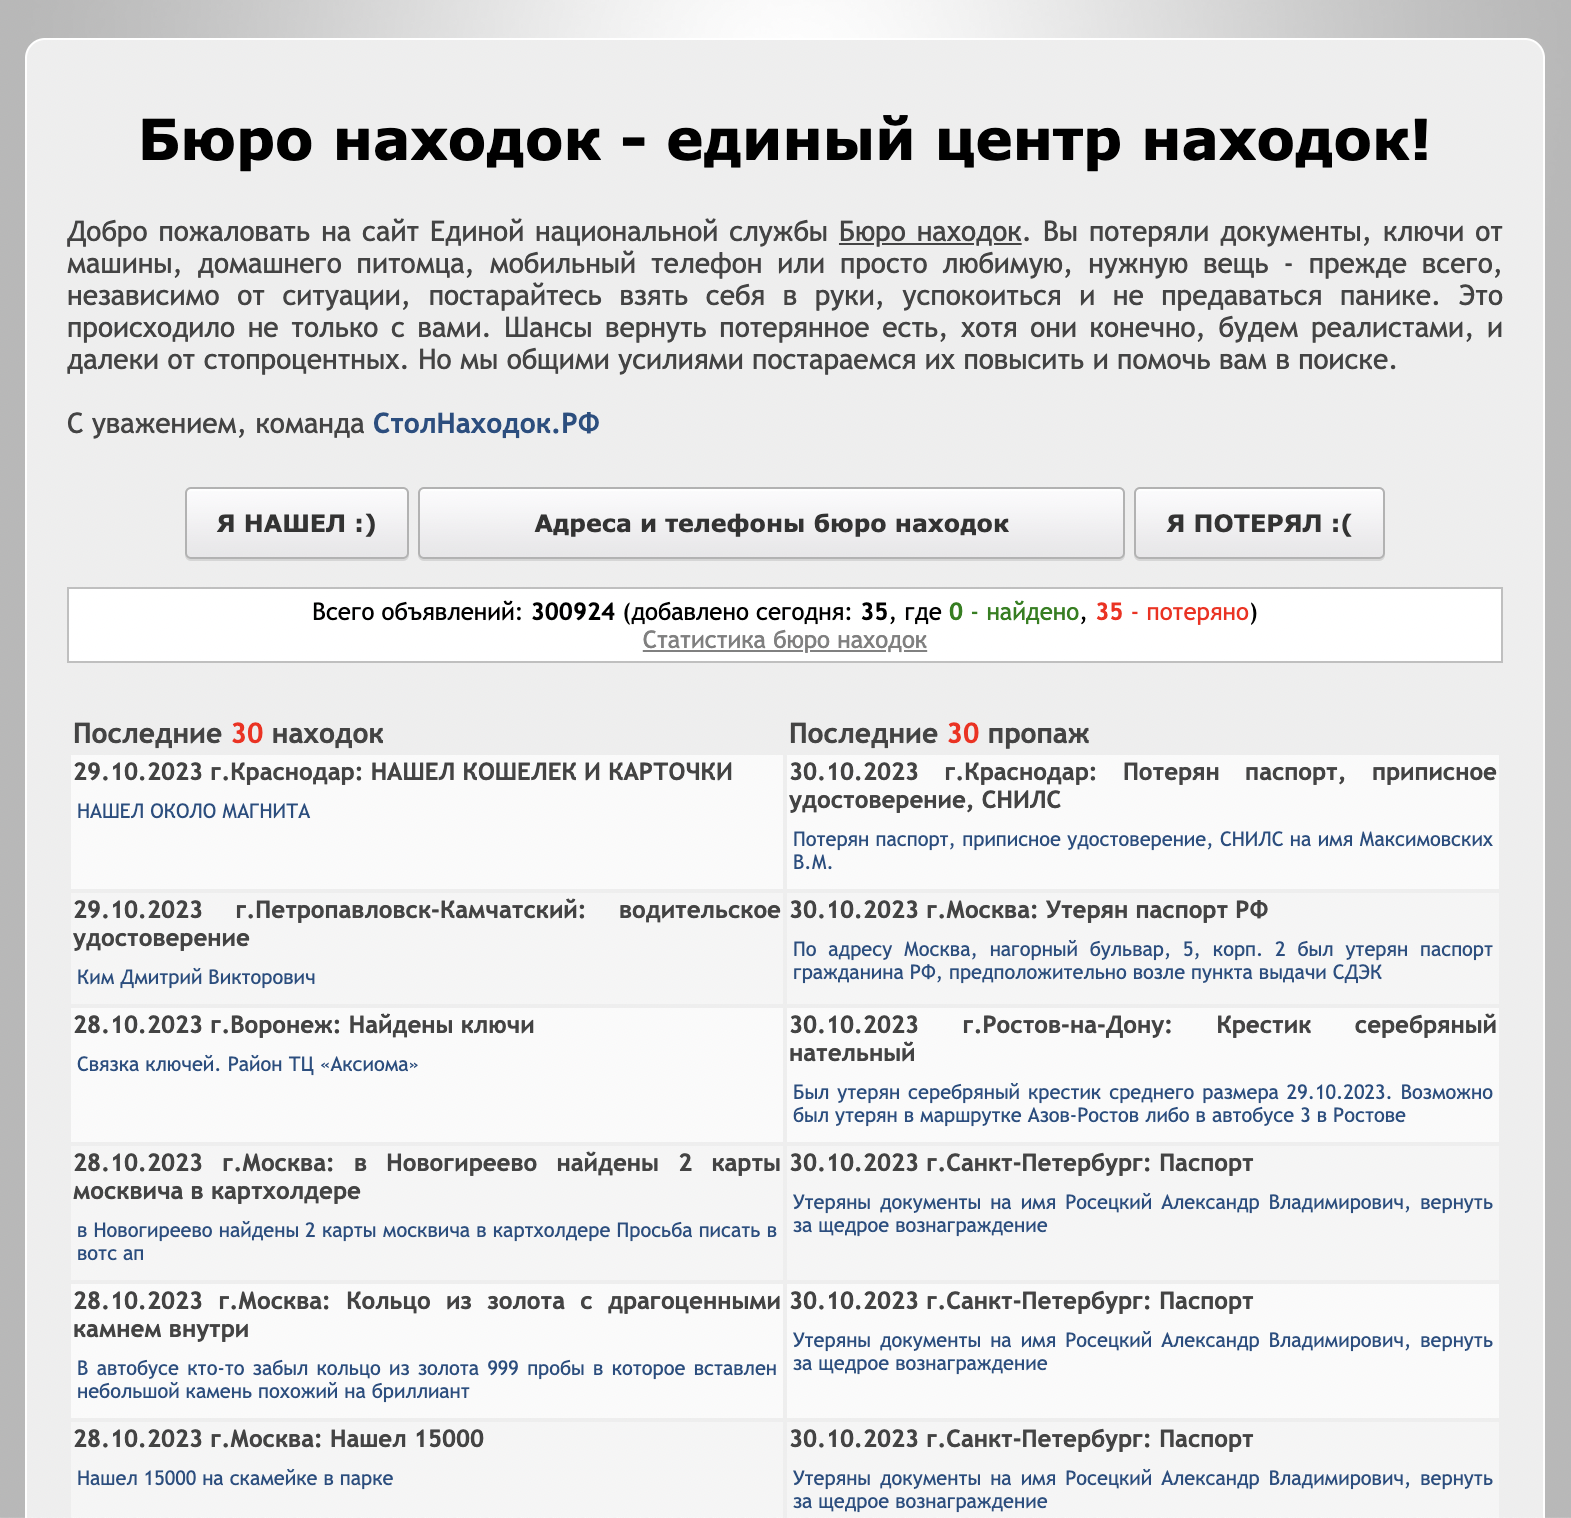
\includegraphics[width=.95\textwidth]{../images/stolNahodok1}
		\parskip=6pt
		\caption{Скриншот системы <<столнаходок.рф>>}
		\label{fig:stolNahodok1}
	\end{figure}
	
	\begin{figure}[htb]
		\centering
		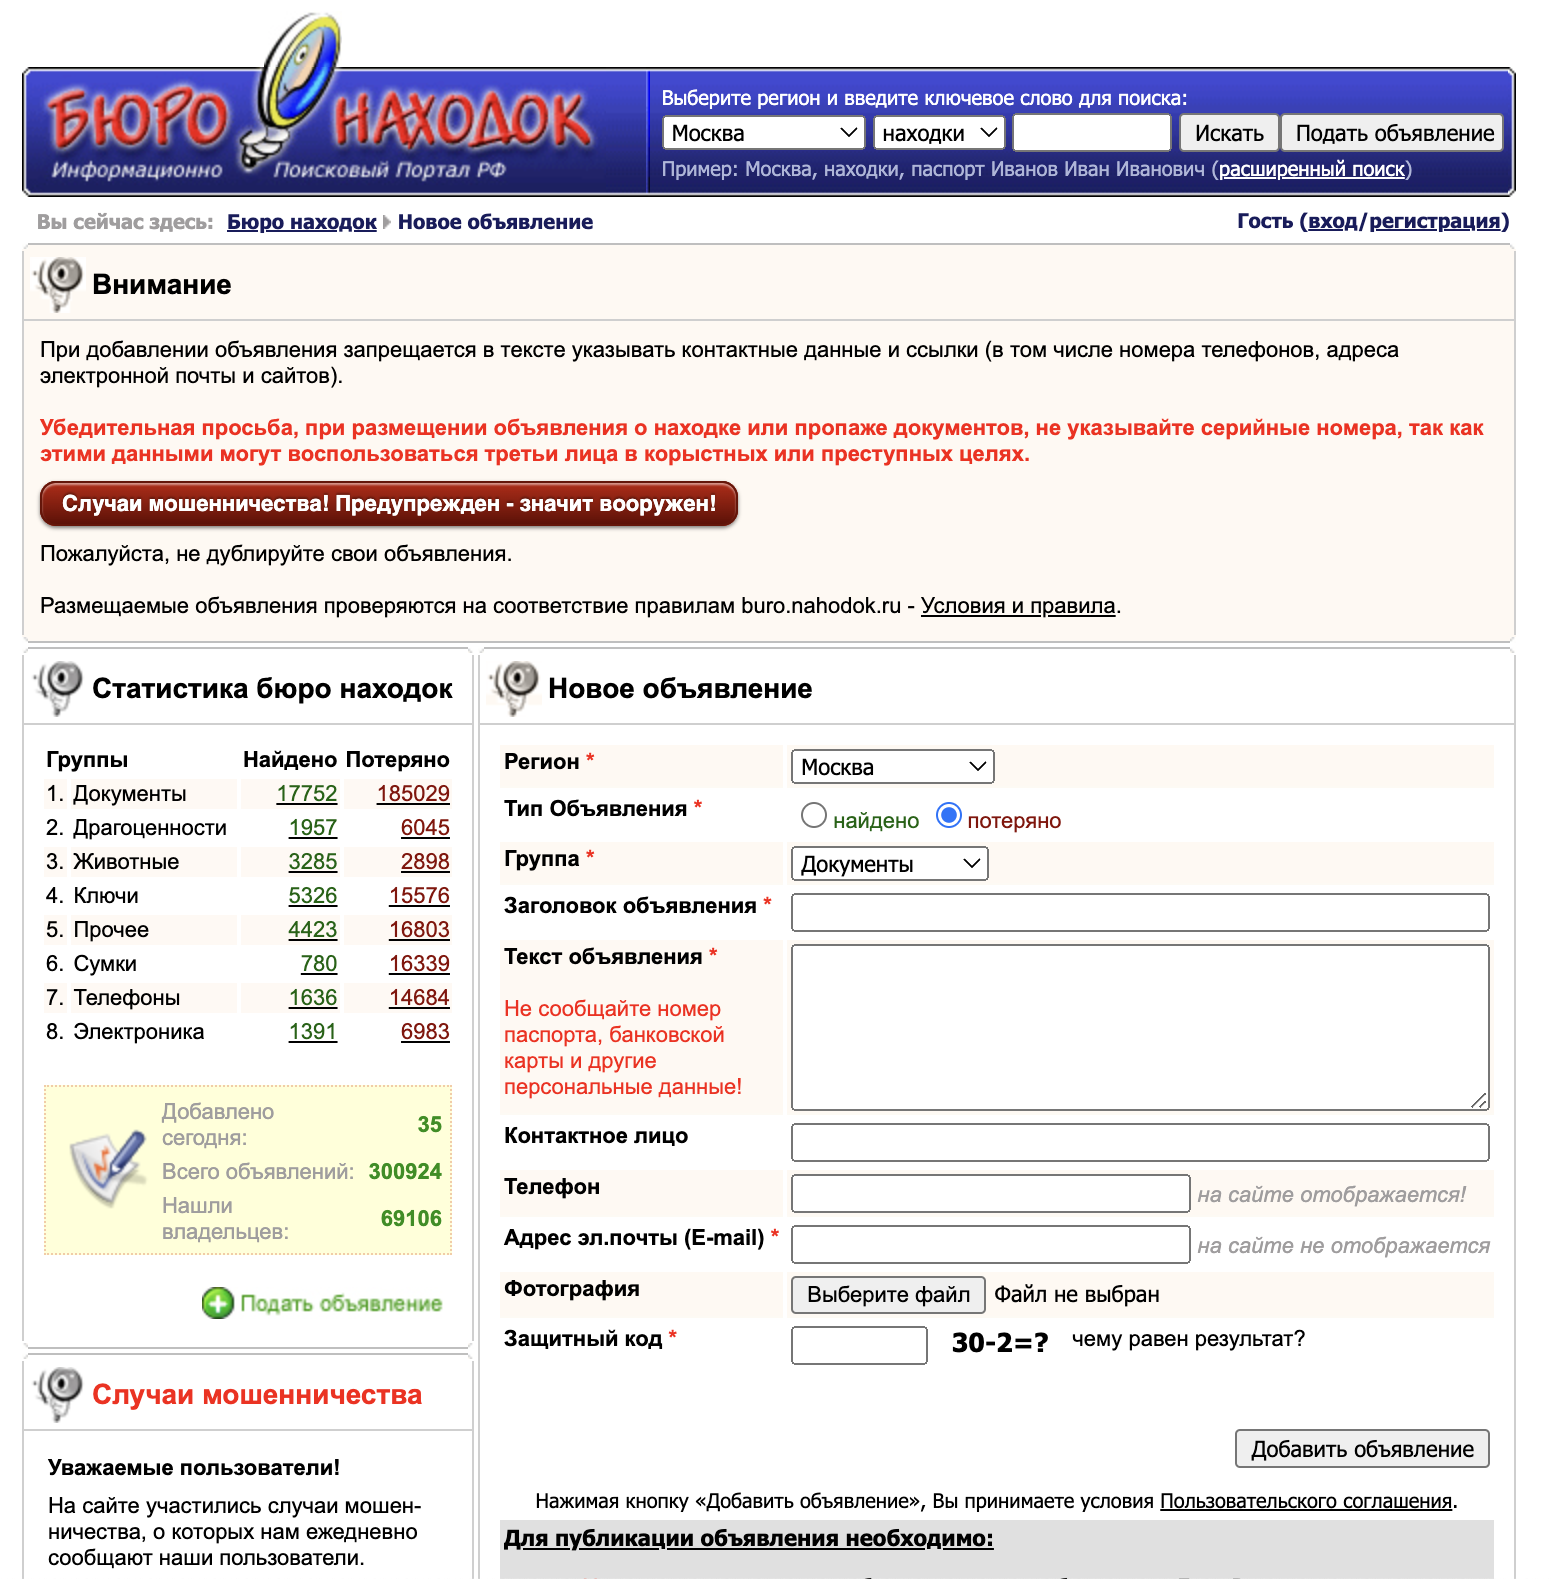
\includegraphics[width=.95\textwidth]{../images/stolNahodok2}
		\parskip=6pt
		\caption{Скриншот системы <<столнаходок.рф>>}
		\label{fig:stolNahodok2}
	\end{figure}
	
	<<Find My Stuff>>~\cite{bib:find_my_stuff} --- это мобильное приложение, разработанное для операционных систем iOS и Android. Оно предлагает функцию отслеживания утерянных предметов через GPS-модуль смартфона, представлено на рис.~\ref{fig:findMyStuff1}, \ref{fig:findMyStuff2}. Пользователи могут отмечать свои вещи на карте и получать уведомления, когда они находятся рядом с утерянным предметом. Однако, ограничение использования только наличием смартфона с GPS-модулем и низкая точность определения местоположения представляют существенные ограничения данного приложения.
	
	\begin{figure}[htb]
		\centering
		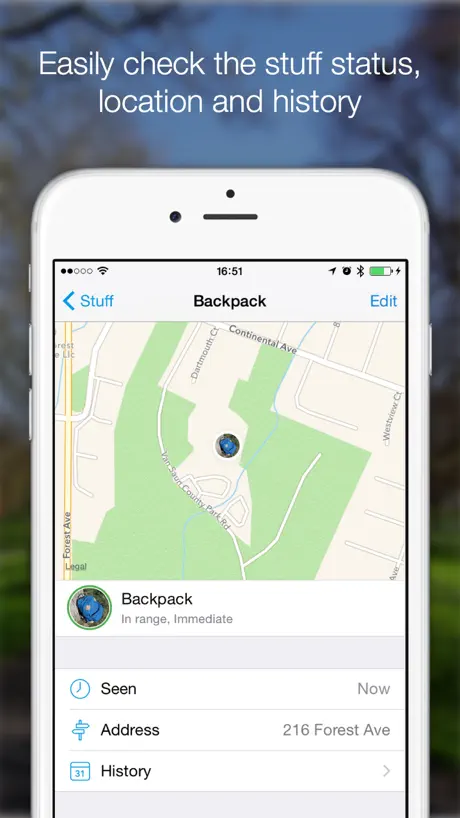
\includegraphics[height=.4\textheight]{../images/findMyStuff1.png}
		\parskip=6pt
		\caption{Скриншот системы <<Find My Stuff>>}
		\label{fig:findMyStuff1}
	\end{figure}
	
	\begin{figure}[htb]
		\centering
		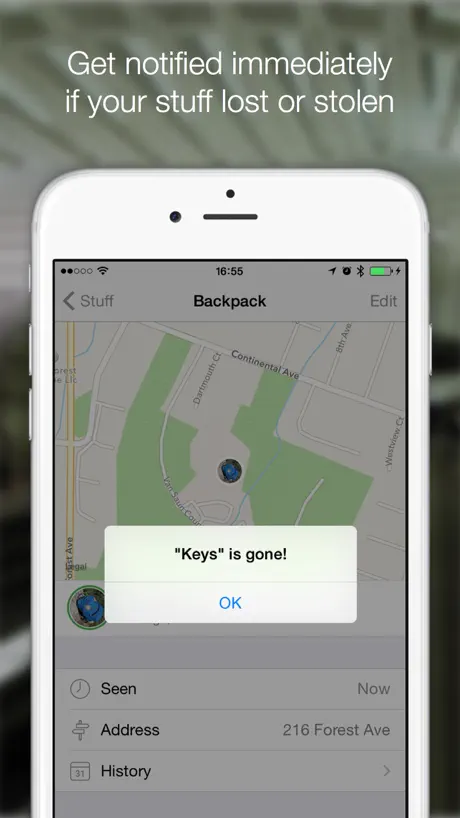
\includegraphics[height=.4\textheight]{../images/findMyStuff2.png}
		\parskip=6pt
		\caption{Скриншот системы <<Find My Stuff>>}
		\label{fig:findMyStuff2}
	\end{figure}
	
	<<Lost Property Office>>~\cite{bib:parliament_lost_and_found} --- это веб-сервис, предоставляемый государственными организациями и органами правопорядка, см. рис.~\ref{fig:lostPropertyOffice}. Сервис позволяет пользователям сообщать о потерянных и найденных предметах, а также предоставляет информацию о процедуре возврата утерянных вещей. Однако, ограниченный доступ к сервису и неудобный процесс регистрации и подачи заявки являются значительными недостатками данного сервиса.
	
	\begin{figure}[htb]
		\centering
		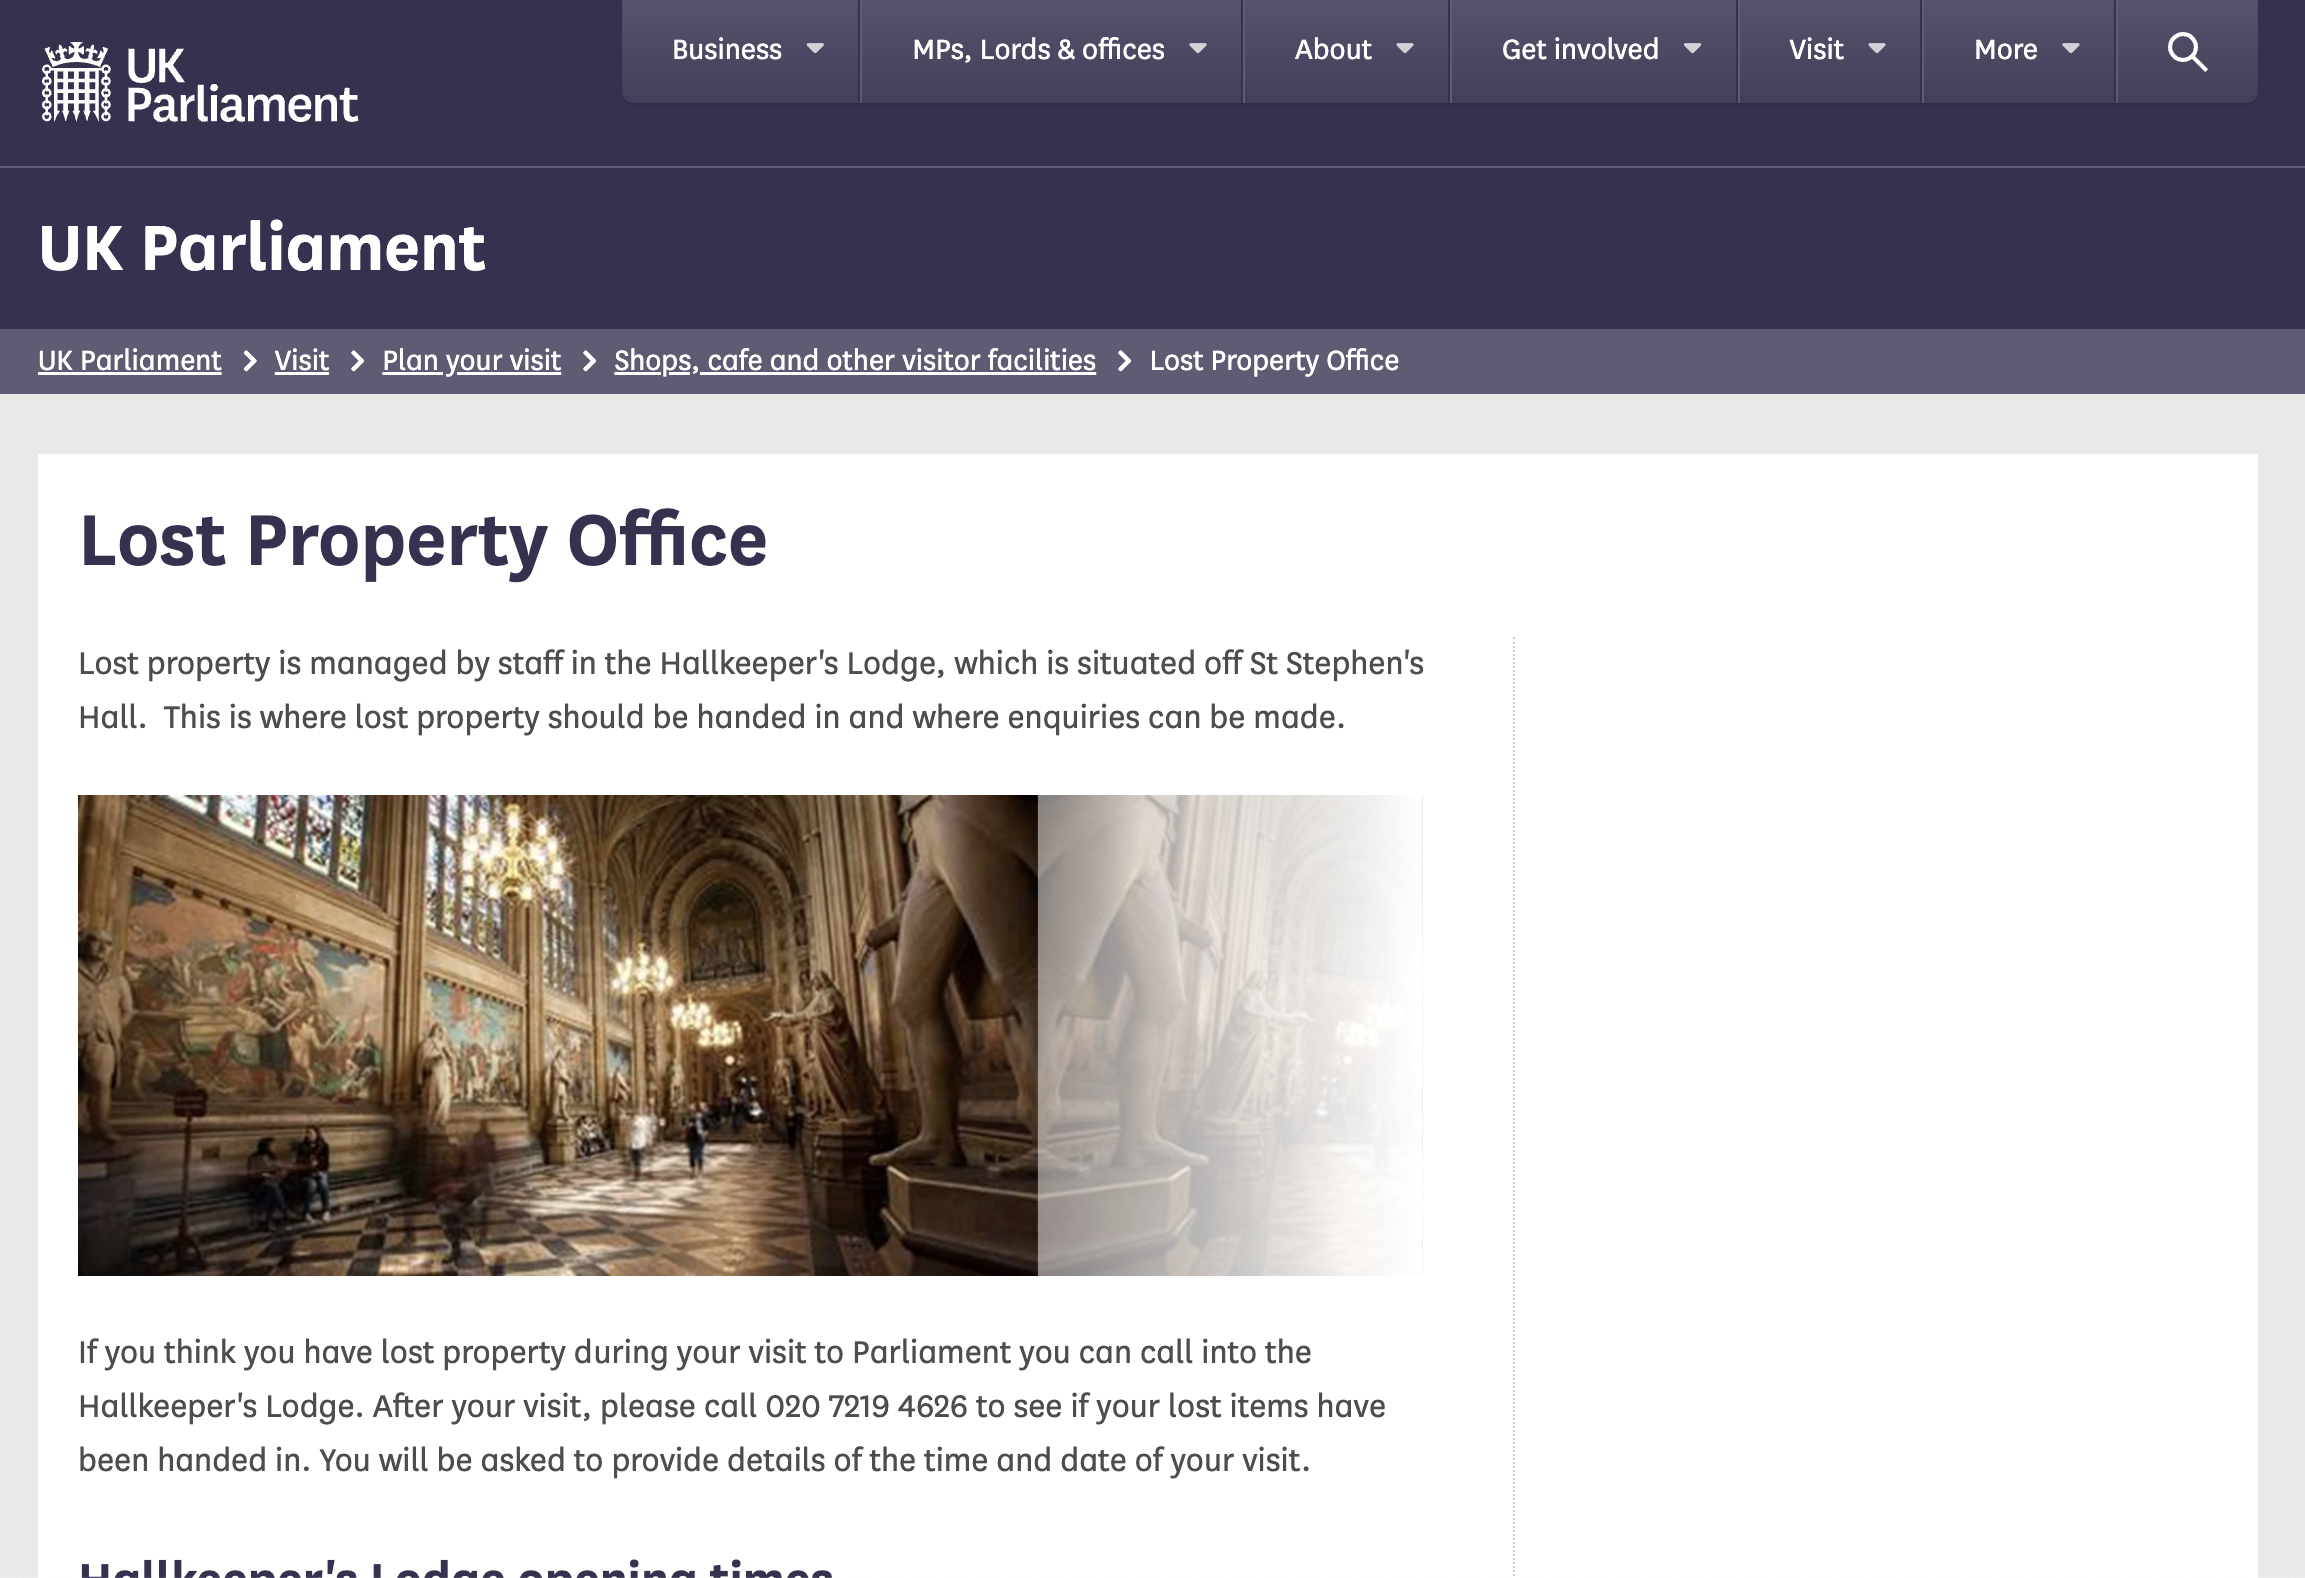
\includegraphics[width=.95\textwidth]{../images/lostPropertyOffice}
		\parskip=6pt
		\caption{Скриншот системы <<Lost Property Office>>}
		\label{fig:lostPropertyOffice}
	\end{figure}
	
	На основании проведенного обзора можно сделать вывод, что существующие веб-сервисы и приложения для поиска и возврата утерянных вещей имеют некоторые преимущества, но также недостатки, которые ограничивают их функциональность и удобство использования. Веб-сервис Бюро находок будет разработан с учетом этих недостатков и предлагать более удобное взаимодействие между пользователями и сервисом.
	
	Ниже приведена сравнительная таблица~\ref{tab:analogs_comparison} основных характеристик и функций приведенных выше аналогов:
	\begin{table}[htb]
		\caption{Сравнительная таблица аналогов}
		\centering
		
		\tolerance=1
		\emergencystretch=10pt
		\hyphenpenalty=1
		\exhyphenpenalty=1
		\small
		\begin{tabular}{ |p{2cm}|p{3cm}|p{2cm}|p{2cm}|p{3cm}|p{2cm}| } 
			\hline
			Сервис~/ Приложение & Интерфейс и удобство использования & Опове\-ще\-ния & Точность определения местоположения & Регистрация и подача заявки & Доступ\-ность \\ \hline
			
			стол\-на\-ходок.рф & Простой и интуитивно понятный интерфейс & Отсут\-ству\-ют & Не\-оп\-ре\-де\-ле\-но & Простой процесс регистрации & Широкий доступ \\ \hline
			
			Find My Stuff & Простой и интуитивно понятный интерфейс & Опо\-ве\-ще\-ния через уведомления & Низкая точность & Простой процесс регистрации & Доступен только на смартфонах с GPS \\ \hline
			
			Lost Property Office & Неудобный процесс регистрации и подачи заявки & Отсут\-ству\-ют & Не\-оп\-ре\-де\-ле\-но & Неудобный процесс регистрации и подачи заявки & Огра\-ни\-чен\-ный доступ \\ \hline
		\end{tabular}
		\label{tab:analogs_comparison}
	\end{table}
	
	\section{Вывод}
	
	В статье проведен детальный анализ существующих веб-ресурсов и приложений, предназначенных для поиска и возвращения утерянных вещей. Были изучены и проанализированы их функциональность, характеристики, преимущества и ограничения.
	
	Одним из наиболее популярных и востребованных решений в данной сфере являются веб-сервисы и приложения "Бюро находок". Они предоставляют пользователям платформу для регистрации утерянных вещей и связи с их владельцами, что упрощает процесс поиска и возвращения потерянных предметов.
	
	
	
	
	\begin{thebibliography}{99\kern\bibindent}
		\bibitem{bib:m24_losts_article} МОСКВА 24 Что теряют москвичи // www.m24.ru: Новости Москвы, репортажи и интервью об основных событиях города URL: \url{https://www.m24.ru/news/gorod/28112019/98853} (дата обращения: 01.09.2023).
		
		\bibitem{bib:usinsk_losts_article} Усинск Онлайн Какие вещи чаще всего теряют россияне // usinsk.online URL: \url{https://usinsk.online/news/kakie-veshhi-chashhe-vsego-teryayut-rossiyane/#:~:text=Чаще%20всего%20россияне%20теряют%3A%20кошельки,1%20процент)%2C%20пишет%20РГ.} (дата обращения: 01.09.2023).
		
		\bibitem{bib:about1} Bataineh, Emad, Bilal Bataineh, and Shama Al Kindi. "Design, development and usability evaluation of an online web-based lost and found system." International Journal of Digital Information and Wireless Communications 5.2 (2015): 75-82. % https://citeseerx.ist.psu.edu/document?repid=rep1&type=pdf&doi=c757d2b9e8b8ba4235342217fab983e2f89f6bd0
		
		\bibitem{bib:about2} Tan, Siok Yee, and Cia Rui Chong. "AN EFFECTIVE LOST AND FOUND SYSTEM IN UNIVERSITY CAMPUS." Management 8.32: 99-112. % http://www.jistm.com/PDF/JISTM-2023-32-09-07.pdf
		
		
		\bibitem{bib:stol_nahodok} Бюро находок // столнаходок.рф: информационно-поисковый портал РФ URL: \url{http://nahodok.ru/} (дата обращения: 01.09.2023).
		
		\bibitem{bib:pona} Потерял Нашел // pona1.ru: бюро находок Пона.рф. Удобный поиск по объявлениям, большая база потерянных вещей и животных URL: \url{https://pona1.ru/sochi} (дата обращения: 01.09.2023).
		
		\bibitem{bib:investopedia_rfid} Investopedia // investopedia.com: Radio Frequency Identification (RFID): What It Is, How It Works URL: \url{https://www.investopedia.com/terms/r/radio-frequency-identification-rfid.asp#:~:text=Radio%20Frequency%20Identification%20(RFID)%20is,checked%20out%20of%20a%20library.} (дата обращения: 01.09.2023).
		
		\bibitem{bib:investopedia_rfid} Investopedia // investopedia.com: Radio Frequency Identification (RFID): What It Is, How It Works URL: \url{https://www.investopedia.com/terms/r/radio-frequency-identification-rfid.asp#:~:text=Radio%20Frequency%20Identification%20(RFID)%20is,checked%20out%20of%20a%20library.} (дата обращения: 01.09.2023).
		
		\bibitem{bib:airtag} AirTag // apple.com: магазин Apple URL: \url{https://www.apple.com/airtag/} (дата обращения: 01.09.2023).
		
		\bibitem{bib:parliament_lost_and_found} Lost Property Office // parliament.uk: веб приложение URL: \url{https://www.parliament.uk/visiting/access/facilities/lost-property/} (дата обращения: 01.09.2023).
	\end{thebibliography}
	
	
	
	\appendix
	
	% Схема базы данных
	%\section{Схема базы данных}

\begin{lstlisting}[label=lst:factorial]
	model Account {
		id                String  @id @default(cuid())
		userId            String
		type              String
		provider          String
		providerAccountId String
		refresh_token     String?
		access_token      String?
		expires_at        Int?
		token_type        String?
		scope             String?
		id_token          String?
		session_state     String?
		user              User    @relation(fields: [userId], references: [id], onDelete: Cascade)
		
		@@unique([provider, providerAccountId])
	}
	
	model Session {
		id           String   @id @default(cuid())
		sessionToken String   @unique
		userId       String
		expires      DateTime
		user         User     @relation(fields: [userId], references: [id], onDelete: Cascade)
		
		@@index([userId], type: Hash)
	}
	
	model User {
		id                String              @id @default(cuid())
		name              String?
		nickname          String              @unique
		socialNetworks    UserSocialNetwork[]
		email             String?             @unique
		emailVerified     DateTime?
		userInfo          String?             @db.VarChar(280)
		role              Role                @default(USER)
		image             String?
		isBlocked         Boolean             @default(false)
		blockReason       String?
		accounts          Account[]
		sessions          Session[]
		lostAndFoundItems LostAndFoundItem[]
		
		@@index([id], type: Hash)
		@@index([nickname], type: Hash)
	}
	
	model VerificationToken {
		identifier String
		token      String   @unique
		expires    DateTime
		
		@@unique([identifier, token])
	}
	
	model UserSocialNetwork {
		id                             String                           @id @default(cuid())
		socialNetwork                  SocialNetwork
		link                           String
		userId                         String
		user                           User                             @relation(fields: [userId], references: [id], onDelete: Cascade)
		lostAndFoundItemSocialNetworks LostAndFoundItemSocialNetworks[]
		
		@@unique([userId, socialNetwork])
		@@index([socialNetwork, userId])
	}
	
	enum Role {
		USER
		MODERATOR
		ADMIN
	}
	
	model LostAndFoundItem {
		id             String                           @id @default(cuid())
		name           String                           @db.VarChar(100)
		description    String                           @default("") @db.VarChar(512)
		campus         Campus
		reason         PostItemReason
		status         LostAndFoundItemStatus           @default(ACTIVE)
		images         String[]
		userId         String
		user           User                             @relation(fields: [userId], references: [id], onDelete: Cascade)
		socialNetworks LostAndFoundItemSocialNetworks[]
		created        DateTime                         @default(now())
		expires        DateTime                         @default(dbgenerated("NOW() + interval '1 week'"))
		
		@@index([id], type: Hash)
	}
	
	enum LostAndFoundItemStatus {
		ACTIVE
		EXPIRED
		BLOCKED
	}
	
	model LostAndFoundItemSocialNetworks {
		id                  String            @id @default(cuid())
		lostAndFoundItemId  String
		lostAndFoundItem    LostAndFoundItem  @relation(fields: [lostAndFoundItemId], references: [id], onDelete: Cascade)
		userSocialNetworkId String
		userSocialNetwork   UserSocialNetwork @relation(fields: [userSocialNetworkId], references: [id], onDelete: Cascade)
		
		@@unique([lostAndFoundItemId, userSocialNetworkId])
	}
	
	enum PostItemReason {
		LOST
		FOUND
	}
	
	enum Campus {
		V78
		S20
		V86
		MP1
		SG22
		SHP23
		U7
	}
	
	enum SocialNetwork {
		TELEGRAM
		VK
	}
\end{lstlisting}
	
	
\end{document}